\section{Notational isomorphism}\label{sec:notational_isomorphism}

Abjad models objects on the page according to common practice notation.

Our musical model attempts to be isomorphic with notation, with one class per
musical construct: \texttt{Note}, \texttt{Rest}, \texttt{Chord},
\texttt{NoteHead}, \texttt{Articulation}, \texttt{TimeSignature}, \texttt{Slur}
and so forth.

[smalltalk?]

\subsection{Notational aggregation}

We assume notational primitives are the elements of composition. The act of
composition then revolves around the iterative aggregation of notational
primitives into arbitrarily complex score objects.

Abjad allows for the iterative aggregation of notational elements via Python's
\emph{mutable sequence} protocol. Score components can be appended, extended or
inserted into other container-like score components.

\begin{lstlisting}
>>> score = Score()
>>> staff_group = StaffGroup()
>>> upper_staff = Staff()
>>> lower_staff = Staff()
>>> score.append(staff_group)
>>> staff_group.extend([upper_staff, lower_staff])
>>> upper_staff.extend("c'4 d'4 e'4 f'4")
>>> lower_staff.extend([Chord("<a ef'>4."), Note("g8")])
>>> lower_staff.insert(0, Rest((1, 2)))
>>> show(score)
\end{lstlisting}

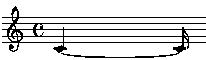
\includegraphics[scale=1.0]{images/section_2_notational_isomorphism-1.pdf}


Note that Abjad makes visualizing notational artifacts simple. Any notational
element or aggregate can be displayed at any time as a PDF via calls to its
top-level \texttt{show()} function in near-publication quality.

Spanners such as slurs, beams and glissandi and indicators such as
articulations and textual directions can be attached to score components via
the \texttt{attach()} function.

\begin{lstlisting}
>>> attach(Slur(), upper_staff[:])
>>> attach(Glissando(), lower_staff[1:])
>>> attach(Articulation('accent'), lower_staff[-1])
>>> show(score)
\end{lstlisting}

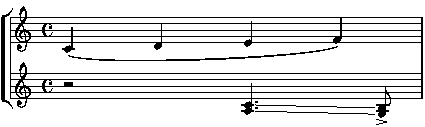
\includegraphics[scale=1.0]{images/section_2_notational_isomorphism-2.pdf}


Abjad attempts to be compositionally agnostic. By providing simple and
unambiguous means of gradually aggregating arbitrarily complex score objects,
we encourage users to develop their own personal approach.

\subsection{Explicit notational modeling}

Abjad models notation explicitly. All notational primitives expressed by Abjad
must conform to the principles of common practice notation. When compositional
inputs cannot be expressed in terms of these principles, we provide affordances
for massaging them into valid notational states.

For example, Abjad expresses the durations of all score components in terms of
rational values -- fractions and integers -- rather than floating point
numbers. Likewise Abjad expresses all pitches in terms of triples of diatonic
note names, accidentals and octave numbers, rather than MIDI numbers or
frequencies. While we provide alternative representations of pitch and rhythm,
as well as affordances for moving between them, the format actually stored in
and used by score components for rendering notation is always the most
notationally-explicit.

\subsection{Written, assignable and prolated durations}

All \texttt{Note}, \texttt{Chord} and \texttt{Rest} objects in Abjad must be
instantiated with a duration corresponding to the written glyphs on the page --
a \emph{written} duration.

Written durations must be \emph{assignable}, a category we invented to model
durational initialization. Durational assignability describes whether a
duration can be represented as a power-of-two flag count combined with zero or
more dots. \texttt{1/4}, \texttt{3/16} and \texttt{7/16} are assignable
durations while \texttt{5/32}, \texttt{9/8} and \texttt{1/12} are not.

Non-assignable durations cannot be represented in common practice notation by a
single glyph. They require two or more glyphs with assignable durations tied
together, for the score component to be tupletted, or both.

Abjad will not automatically render a single note with a duration of
\texttt{5/16} as two or more notes tied together. We consider such behavior to
be too implicit. There are too many potentially compositionally valid ways to
render a duration such as \texttt{5/16} into a series of tied assignable
durations: \texttt{1/4 + 1/16}, \texttt{3/16 + 2/16}, \texttt{2/16 + 3/16},
\texttt{1/16 + 1/4}, \texttt{1/8 + 1/8 + 1/16} etc. Instead we provide
affordances for generating tied notes from non-assignable durations. One such
affordance is our \texttt{scoretools.make\_notes()} function, which chooses
smart defaults for generating tied glyphs from otherwise un-notateable input.

\begin{lstlisting}
>>> selection = scoretools.make_notes("c'", [(5, 16)])
>>> staff = Staff(selection)
>>> show(staff)
\end{lstlisting}

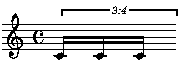
\includegraphics[scale=1.0]{images/section_2_notational_isomorphism-3.pdf}


All score components also have a \emph{prolated} duration - the product of
their written duration and their \emph{prolation}. Prolation is the cumulative
product of all the \emph{multiplier} of every tuplet found in the
\emph{parentage} of a score component. A score component's prolation depends on
its location in the score hierarchy, and is not an inherent property of itself
independent that hierarchy.

Three \texttt{Note} objects each having a prolated duration of \texttt{1/12}
can be represented as either three \texttt{1/16} notes in a \texttt{3:4} tuplet
or as three \texttt{1/8} notes in a \texttt{3:2} tuplet. As all Abjad
\texttt{Note} objects must have an assignable written duration, the three notes
above must have written durations of either \texttt{1/8} or \texttt{1/16}, and
the tuplet must be correspondingly an explicit diminution or augmentation to
provide the desired prolation of \texttt{2/3} or \texttt{4/3}.

\begin{lstlisting}
>>> selection = scoretools.make_notes("c'", [(1, 12)] * 3)
>>> tuplet = selection[0]
>>> show(tuplet)
\end{lstlisting}

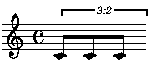
\includegraphics[scale=1.0]{images/section_2_notational_isomorphism-4.pdf}

\begin{lstlisting}
>>> tuplet.toggle_prolation()
>>> show(tuplet)
\end{lstlisting}

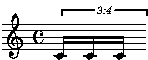
\includegraphics[scale=1.0]{images/section_2_notational_isomorphism-5.pdf}


The durational information of any aggregate score object in Abjad is therefore
always explicit and unambiguous with regard to its notational reality.